\section*{Exercises 6.4}
%
\begin{enumerate} 
\item In our definition of the composition of two functions,  $f$  and  $g$, we required that the domain of  $g$  be equal to the codomain of  $f$.  However, it is sometimes possible to form the composite function  $g \circ f$ even though  
$\text{dom}( g ) \ne \text{codom}( f )$.  For example, let
\label{exer:sec64-1}
\begin{center}
\begin{tabular}{l l l}
$f\x \mathbb{R} \to \mathbb{R}$  &  be defined by	 &  $f( x ) = x^2  + 1$, and let \\
$g\x \mathbb{R} - \left\{ 0 \right\} \to \mathbb{R}$  &  be defined by & 
$g( x ) = \dfrac{1}{x}$. \\
\end{tabular}
\end{center}

\begin{enumerate}
  \item Is it possible to determine  $( {g \circ f} )( x )$  for all  
        $x \in \mathbb{R}$?  Explain.

  \item In general, let  $f\x A \to T$ and  $g\x B \to C$.  Find a condition on the domain of  $g$               (other than  $B = T$)  that results in a meaningful definition of the composite function  
   $g \circ f\x A \to C$.
\end{enumerate}


\xitem Let  $h\x \mathbb{R} \to \mathbb{R}$ be defined by  $h( x ) = 3x + 2$ and  $g\x \mathbb{R} \to \mathbb{R}$ be defined by  $g( x ) = x^3 $.  Determine formulas for the composite functions  $g \circ h$  and  $h \circ g$.  Is the function $g \circ h$ equal to the function $h \circ g$?  Explain.  What does this tell you about the operation of composition of functions? \label{exer64:notcommutative}




\xitem Following are formulas for certain real functions.  Write each of these real functions as the composition of two functions.  That is, decompose each of the functions. \label{exer:sec64-2}

\begin{multicols}{2}
\begin{enumerate}
\item $F( x ) = \cos ( {e^x } )$

\item $G( x ) = e^{\cos ( x )} $

\item $H( x ) = \dfrac{1}{{\sin x}}$

\item $K( x ) = \cos \!\left( {e^{ - x^2 } } \right)$
\end{enumerate}
\end{multicols}


\item The \textbf{identity function}
\index{identity function}%
 on a set  $S$, denoted by $I_S$,  is defined as follows: \linebreak  $I_S \x S \to S$ by  $I_S ( x ) = x$
for each  $x \in S$. \label{exer:sec64-4}  Let  $f\x A \to B$.

\begin{enumerate}
\yitem For each  $x \in A$, determine   $( {f \circ I_A } )( x )$ and use this to prove that  $f \circ I_A  = f$.

\item Prove that  $I_B  \circ f = f$\!.
\end{enumerate}


\item \label{exer:sec64-3} \begin{enumerate} 
\yitem Let  $f\x \mathbb{R} \to \mathbb{R}$ be defined by  
$f( x ) = x^2 $,  let $g\x \mathbb{R} \to \mathbb{R}$ be defined by  
$g( x ) = \sin x$, and let $h\x \mathbb{R} \to \mathbb{R}$ be defined by  
$h( x ) = \sqrt[3]{x}$.  
\vskip10pt
Determine formulas for    $\left[ ( {h \circ g} ) \circ f \right] ( x )$ and  $\left[ h \circ ( {g \circ f} ) \right] ( x )$.  
\vskip10pt
Does this prove that  $( {h \circ g} ) \circ f = h \circ ( {g \circ f} )$
for these particular functions?  Explain.

\item Now let $A$, $B$, $C$, and $D$ be sets and let  $f\x A \to B$,  $g\x B \to C$,  and  $h\x C \to D$.  Prove that  
$( {h \circ g} ) \circ f = h \circ ( {g \circ f} )$.  That is, prove that function composition is an associative operation.
\end{enumerate}


\xitem Prove Part~(\ref{T:compositefunctions1}) of Theorem~\ref{T:compositefunctions}.
\label{exer:compositefunctions1}

Let  $A$, $B$, and  $C$  be nonempty sets and let  $f\x A \to B$  and  $g\x B \to C$.  If  $f$  and  $g$  are both injections, then  $g \circ f$  is an injection. \label{exer:sec64-5}


\item For each of the following, give an example of functions  $f\x A \to B$ and \linebreak
$g\x B \to C$ that satisfy the stated conditions, or explain why no such example exists. 
\label{exer:sec64-8}

\begin{enumerate}
\yitem The function  $f$  is a surjection, but the function  $g \circ f$  is not a surjection.

\yitem The function  $f$  is an injection, but the function  $g \circ f$  is not an injection.

\item The function  $g$  is a surjection, but the function  $g \circ f$  is not a surjection.

\item The function  $g$  is an injection, but the function  $g \circ f$  is not an injection.

\item The function  $f$  is not a surjection, but the function  $g \circ f$  is a surjection.

\yitem The function  $f$  is not an injection, but the function  $g \circ f$  is an injection.

%\item The function  $f$  is not a surjection, but the function $g \circ f$  is a surjection.

\item The function  $g$  is not a surjection, but the function $g \circ f$  is a surjection.

\item The function  $g$  is not an injection, but the function $g \circ f$  is an injection.
\end{enumerate}


\item Let $A$ be a nonempty set and let $f\x A \to A$.  For each $n \in \N$, define a function 
$f^n\x A \to A$ recursively as follows:  $f^1 = f$ and for each $n \in \N$, 
$f^{n+1} = f \circ f^n$.  For example, $f^2 = f \circ f^1 = f \circ f$ and 
$f^3 = f \circ f^2 = f \circ ( f \circ f )$.
\begin{enumerate}
\item Let $f\x  \R \to \R$ by $f(x) = x + 1$ for each $x \in \R$.  For each $n \in \N$ and for each $x \in \R$, determine a formula for $f^n(x)$ and use induction to prove that your formula is correct.

\item Let $a, b \in \R$ and let $f\x  \R \to \R$ by $f(x) = ax + b$ for each $x \in \R$.  For each $n \in \N$ and for each $x \in \R$, determine a formula for $f^n(x)$ and use induction to prove that your formula is correct.

\item Now let $A$ be a nonempty set and let $f\x A \to A$.  Use induction to prove that for each $n \in \N$, $f^{n+1} = f^n \circ f$.  (\note  You will need to use the result in Exercise~(\ref{exer:sec64-3}).)
\end{enumerate}
\end{enumerate}



\subsection*{Explorations and Activities}
\setcounter{oldenumi}{\theenumi}
\begin{enumerate} \setcounter{enumi}{\theoldenumi}
  \item \textbf{Exploring Composite Functions}.  \label{exer:exploringcomposite}
Let  $A$, $B$, and  $C$  be nonempty sets and let  $f\x A \to B$  and  $g\x B \to C$.  For this activity, it may be useful to draw your arrow diagrams in a triangular arrangement as follows:
\begin{figure}[h]
\begin{center}
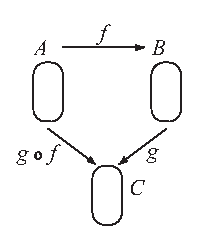
\includegraphics{figps-comparrow.eps}
%\caption{Composition of Functions} \label{fig:functioncomposition2}
\end{center}
\end{figure}

It might be helpful to consider examples where the sets are small.  Try constructing examples where the set $A$ has 2 elements, the set $B$ has 3 elements, and the set $C$ has 2 elements.

\begin{enumerate}
\item Is it possible to construct an example where  $g \circ f$  is an injection,  $f$  is an injection, but  
$g$  is not an injection?  Either construct such an example or explain why it is not possible.  %\hint  It might be helpful to consider examples where the sets are small.  Try constructing examples where the set $A$ has 2 elements, the set $B$ has 3 elements, and the set $C$ has 2 elements.

\item Is it possible to construct an example where  $g \circ f$  is an injection,  $g$  is an injection, but  $f$  is not an injection?  Either construct such an example or explain why it is not possible.  %\hint Try working with sets given in the hint in part~(a).

\item Is it possible to construct an example where  $g \circ f$  is a surjection,  $f$  is a surjection, but  $g$  is not a surjection?  Either construct such an example or explain why it is not possible.  

\item Is it possible to construct an example where  $g \circ f$  is surjection,  $g$  is a surjection, but  $f$  is not a surjection?  Either construct such an example or explain why it is not possible.
\end{enumerate}


\item \textbf{The Proof of Theorem~\ref{T:morecompositefunctions}}.  Use the ideas from 
Exercise~(\ref{exer:exploringcomposite}) to prove Theorem~\ref{T:morecompositefunctions}.  
\label{exer:morecompositefunctions1}
Let  $A$, $B$, and  $C$  be nonempty sets and let  $f\x A \to B$  and  $g\x B \to C$.  
\begin{enumerate}
\item If  $g \circ f\x A \to C$  is an injection, then  $f\x A \to B$  is an injection. \label{exer:sec64-6}


\item If  $g \circ f\x A \to C$  is a surjection, then  $g\x B \to C$  is a surjection. \label{exer:sec64-7}
\end{enumerate}

\hint For part~(a), start by asking, ``What do we have to do to prove that $f$ is an injection?''  Start with a similar question for part~(b).

\end{enumerate}


\hbreak

\endinput









\endinput
